+++Motivate motivate motivate+++\\
Nonlinear evolution equations ubiquitous across the sciences. These typically take the form 
$$ \dot{x} = F(x)$$ where $x\in \mathbf{R}^n, F\in C^r(\mathbf{R}^n,\mathbf{R}^n)$. We will be interested in systems that occur on different timescales, known as fast-slow systems. These occur naturally in physics, neuroscience and many other biological scenarios. +++ Van der Pol, FitzHugh-Nagumo, other bio ref?+++.\\
Fast-slow systems are systems of differential equations that can be viewed on two different time scales, which are separated by a parameter.

We will first study two dimensional systems, with one fast and one slow variable, with a separation in speed of $\epsilon$.
These systems are generally of the form
\begin{align} 
\begin{cases}
x' &=\frac{dx}{dt}= f(x,y,\lambda, \epsilon),\\
y' &= \frac{dy}{dt}= \epsilon g( x,y, \lambda, \epsilon),
\end{cases}\label{FastS}
\end{align}
which is known as the fast system.
If time is `slowed down' using a scaling $t = \frac{\tau}{\epsilon} $, we find that this can be rewritten as
\begin{align}
\begin{cases}
\epsilon \dot{x} &= \epsilon \frac{dx}{d \tau} = f(x,y,\lambda, \epsilon),\\
\dot{y} & = \frac{dy}{d \tau} =  g( x,y, \lambda, \epsilon),
\end{cases}\label{SlowS}
\end{align}
which is called the slow system.\\

Here $x$ is called the fast variable, while $y$ is the slow variable. In our case the parameter $\lambda\in \R $ will control the location of the equilibrium of the system (see Section \ref{sec:canard-points}), although it can also be considered as a constant. The time scale separation parameter, $\epsilon$ is much less than 1. Indeed, if $\epsilon=1$, this system is no longer fast-slow as both variables change on the same timescale. The functions $f$ and $g$ are required to be $r+1$ differentiable \st we have $f,g \in  C^{r+1} $, where $ r $ is the number of dimensions present. There is no restriction on the number of timescales. It is possible to have three or more time scales, separated by additional parameters, as well as more state-space variables (See Section \ref{sec:MMO}). \\

Throughout what follows, the motivating example will be the Van der Pol equation. The Van der Pol oscillator is a well-studied second order ODE that is used to model a variety of physical and biological phenomena. It was developed by the Dutch physicist and electrical engineer Balthasar Van der Pol, who conducted research on electrical circuits. In certain cases, he observed stable oscillations later named relaxation oscillations. This equation can be scaled so that it becomes a fast-slow system of the form shown in Equation\ref{FastS} after a change of variables.

\subsection{Derivation of the Van der Pol Fast-Slow System}

The Van der Pol Oscillator describes the evolution of the position coordinate \(x(t)\) according to the following the ODE:
\begin{equation} \label{eq:vdP}
\ddot{x}(t)-\mu\left(1-x^2(t)\right)\dot{x}(t)+x(t)=0,   
\end{equation}
where \(\mu \gg 1\) is a scalar constant. \\

In order to analyse systems (\ref{FastS}) and (\ref{SlowS}) using Geometric Singular Pertubation Theory (GSPT), the singular limit $\epsilon \to 0$ is considered:

\begin{align} \label{FastS0}
\begin{cases}
x' &=\frac{dx}{dt}= f(x,y,\lambda, \epsilon)\\
y' &= 0,
\end{cases}
\end{align}
which is called the layer problem, and
\begin{align}\label{SlowS0}
\begin{cases}
0 &= \epsilon \frac{dx}{d \tau} = f(x,y,\lambda, 0)\\
\dot{y} & = \frac{dy}{d \tau} =  g( x,y, \lambda,0),
\end{cases}
\end{align}
called the reduced system.\\

Fast- Slow systems are systems of differential equations that can be viewed on two different time scales, which are separated by a parameter.
These systems are generally of the form
\begin{align} 
\begin{cases}
x' &=\frac{dx}{dt}= f(x,y,\lambda, \epsilon),\\
y' &= \frac{dy}{dt}= \epsilon g( x,y, \lambda, \epsilon),
\end{cases}\label{FastS}
\end{align}
which is known as the fast system.
Using a scaling for the time, $t = \frac{\tau}{\epsilon} $, we find that this can be rewritten as
\begin{align}
\begin{cases}
\epsilon \dot{x} &= \epsilon \frac{dx}{d \tau} = f(x,y,\lambda, \epsilon),\\
\dot{y} & = \frac{dy}{d \tau} =  g( x,y, \lambda, \epsilon),
\end{cases}\label{SlowS}
\end{align}
which is called the slow system.\\

Here $x$ is called the fast variable, while $y$ is the slow variable. $\lambda$ is a parameter (see Section \ref{sec:canard-points}), $\epsilon$ is the time scale separation parameter and satisfies $0< \epsilon << 1$. The functions $f$ and $g$ are required to be sufficiently smooth \st we have $ C^{r+1} $ smoothness, where $ r $ is the number of dimensions present. It is generally possible to have three or more time scales, separated by additional parameters, as well as more state-space variables. \\

In order to analyse systems (\ref{FastS}) and (\ref{SlowS}) using Geometric Singular Pertubation Theory (GSPT), the singular limit $\epsilon \to 0$ is considered:

\begin{align} \label{FastS0}
\begin{cases}
x' &=\frac{dx}{dt}= f(x,y,\lambda, \epsilon)\\
y' &= 0,
\end{cases}
\end{align}
which is called the layer problem, and
\begin{align}\label{SlowS0}
\begin{cases}
0 &= \epsilon \frac{dx}{d \tau} = f(x,y,\lambda, 0)\\
\dot{y} & = \frac{dy}{d \tau} =  g( x,y, \lambda,0),
\end{cases}
\end{align}
called the reduced system.\\

Now considering Equation \ref{SlowS0}, we can write $f(x,y,\lambda, 0)=0$. Then we are able to define the critical manifold as:,
\begin{align} \label{CriticalS}
S= \left\{ (x,y) : f(x,y,\lambda, 0)=0 \right \},
\end{align}
where, by definition of $S$, the points $(x,y) \in S$ are equilibria of (\ref{FastS0}). Before we continue, it is useful to have a visual interpretation of these flows, 
\begin{figure}[h!]\centering

	\begin{subfigure}[t]{0.45\textwidth}
		\centering
		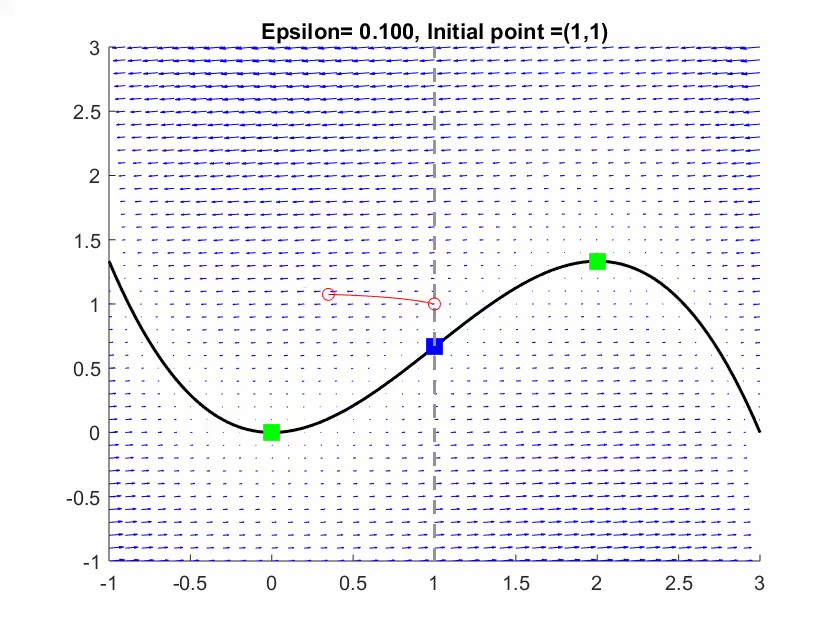
\includegraphics[width=.8\linewidth]{vdPhopf-Moment-1.jpg}
		\caption{The initial flow within the system starting at $ (x,y)=(1,1) $.} 
	\end{subfigure}
	\hfill
	\begin{subfigure}[t]{0.45\textwidth}
		\centering
		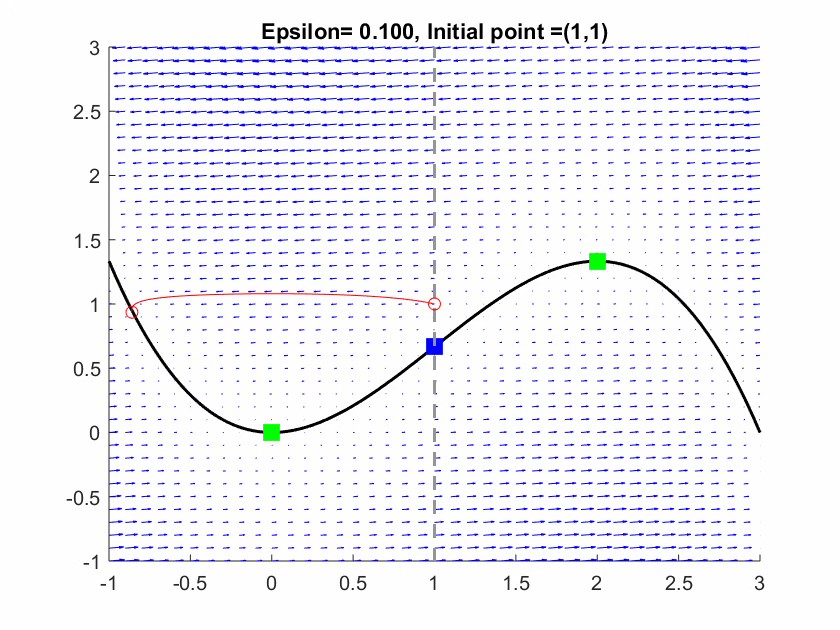
\includegraphics[width=.8\linewidth]{vdPhopf-Moment-2.jpg}
		\caption{The flow as it hits the slow manifold.} 
	\end{subfigure}
	
	\vspace{1cm}
	\begin{subfigure}[t]{0.45\textwidth}
		\centering
		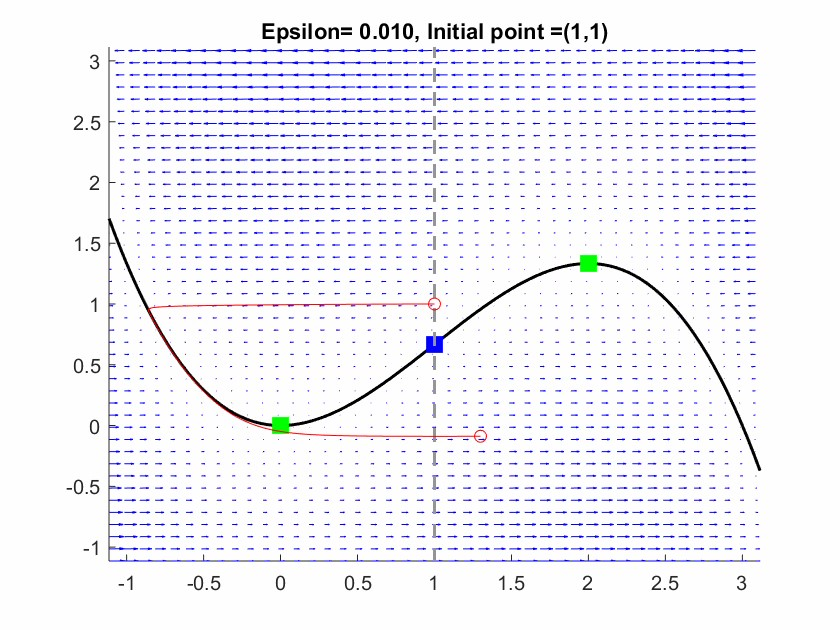
\includegraphics[width=.8\linewidth]{vdp-jump1}
		\caption{The flow as it intersects with the fold point and begins the jump.} 
	\end{subfigure}
	\hfill
	\begin{subfigure}[t]{0.45\textwidth}\centering
		% just an empty subfigure to shift C below A
		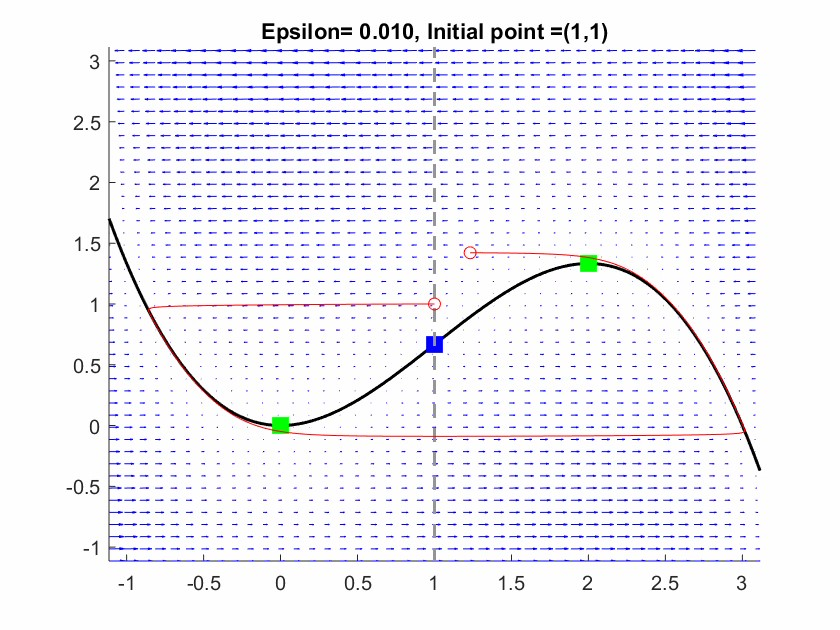
\includegraphics[width=.8\linewidth]{vdp-jump2}
		\caption{The second jump before continuing in a periodic fashion.}
	\end{subfigure}
	\caption{Flows in the \vdp system.}
	\label{fig: vdp flow diagram}
\end{figure}\newline
where we can see that the flows will travel towards our fold point, following the relevant branches. It is worth noting that our flow does not meet the fold point exactly, although this is an `error', it does not directly effect our simulations - as is discussed in Section \ref{sec:matlab-stuff}.


